\documentclass{article}
\usepackage{enumitem}
\usepackage{graphicx}
\usepackage{array}
\usepackage{amsmath}\usepackage{hyperref}
\graphicspath{ {report figures/} }
\usepackage{titlesec}
\usepackage[margin=1.5in]{geometry}
\geometry{a4paper, top=30mm, bottom=30mm}
\titleformat*{\section}{\large\bfseries}
\setlength{\skip\footins}{1cm}
\date{}
\begin{document}
\title{\vspace{-1cm}Part 2: System Requirement Specification}
\maketitle
\section{Project Scope}
Most Australian land is underpopulated except for a few major cities. Therefore the health infrastructures and health practitioners are sparsely distributed in these region. To solve this problem for the residents in these regions, building facilities and relocating health practitioners are costly and time consuming. A remote consultation and diagnostic system can save residents a lot of time in traveling. When surgery and physiotherapy are not necessary, patients can receive prescription and medicine remotely from the system. This would be the most cost efficient way to easy the inconvenience of accessing healthcare resources in remote regions.\\\\
This project will focus on designing a remote healthcare access system (RHAS) to counter the geographical gap between rural and remote communities and major cities. With the RHAS, people living in remote area in Australia can receive timely medical consultations, diagnostics, and self-administered drug treatments, improving their overall health conditions. More details about the scope of the project are listed below:
\begin{itemize}
\item \textbf{Assumptions and Constrains}\\
There are a few assumptions that the table research is based on. Some constrains are found during the research of the project scope as well. Both of them can be found in appendix 1.
\item \textbf{Context Diagram}\\
To roughly delineate the boundary of RHAS, identify stakeholders, subsystems and their relationships, a context diagram is drawn in appendix 2.
\item \textbf{Stakeholders List}\\
A stakeholder analysis is conducted to rank all stakeholders of this project in a list which can be found in appendix 3.
\item \textbf{Needs List}\\
The description and importance of needs from high-importance stakeholders are researched and listed in the appendix 4.
\end{itemize}
\section{Requirements List}
\begin{itemize}[label={}]
\item \textbf{R1} The RHAS shall be available in \textit{rural and remote area listed in MMM standard}.
\item \textbf{R1.1} The RHAS shall be available on \textit{intended platforms}
\item \textbf{R1.2} The RHAS shall be available in conditions where internet or smart devices are inaccessible
\item \textbf{R1.2.1} The RHAS shall be available via phone call
\item \textbf{R1.3} The RHAS shall include a remote payment system.
\item \textbf{R1.3.1} The remote payment system shall provide an interface for users to claim benefit from medicare.
\item \textbf{R1.3.2} The remote payment system shall provide an interface for users to claim benefit from \textit{major health insurance providers}.
\item \textbf{R1.3.3} The payment system shall be capable to make payments for medicine.
\item \textbf{R1.3.4} The payment system shall be capable to make payments for \textit{intended medical services}.
\item \textbf{R2} The RHAS shall provide \textit{intended medical services}.
\item \textbf{R2.1} The RHAS shall provide diagnostic services.
\item \textbf{R2.1.1} Diagnostic services must be provided from \textit{registered health practitioners}.
\item \textbf{R2.2} The RHAS shall provide consultation services.
\item \textbf{R2.2.1} Consultation services must be provided from \textit{registered health practitioners}.
\item \textbf{R2.3} The RHAS shall provide medicine prescription services.
\item \textbf{R2.3.1} Prescription services must be provided from \textit{registered health practitioners}.
\item \textbf{R2.4} The RHAS shall include a medicine supply network.
\item \textbf{R2.4.1} The medicine supply network must comply with the National Health Act 1953 for prescriptions of PBS or RPBS medicines regulations (Pharmaceutical Society Of Australia, n.d.).
\item \textbf{R2.4.2} The medicine supply network shall be capable to deliver medicines to all \textit{rural and remote area listed in MMM standard} with 2 days.
\item \textbf{R2.4.2.1} The medicine supply network should deliver medicine from closest pharmacy to the user.
\item \textbf{R2.4.2.2} The medicine supply network should build medicine storage where deliveries of medicine cannot be guaranteed in 2 days from closest pharmacy.\\
\end{itemize}
The hierarchical relationship of the requirements and their corresponding needs are shown in the requirements breakdown structure below:
\begin{figure}[h]
    \centering
    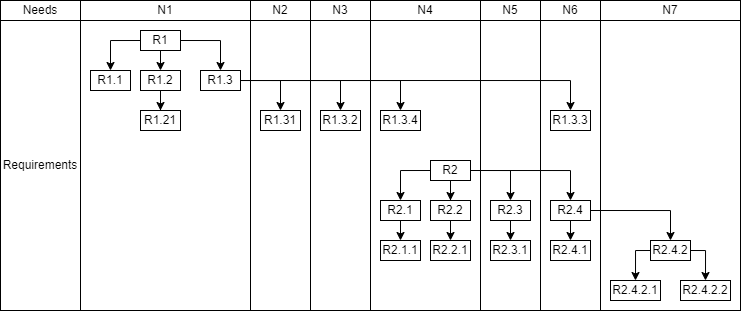
\includegraphics[scale=0.5]{RBS}
    \label{1-2-a}
\end{figure}
\section{Recommendation}
The prospect for designing the RHAS is great according to the analysis in this report. First of all, the design team now have a clearly defined scope of what the project should include and achieve. Despite that there are some constrains about the services RHAS can provide, it is still a significant improvement to the availability of healthcare in rural and remote areas in Australia. \\\\
Secondly, stakeholders have provided reasonable needs which can be interpreted into clear feasible consistent and objective requirements. This means engineers will fully understand what stakeholders want and thus make decisions that meets their needs. In addition, once the prototype is successfully designed, the design team will be able to validate the performance of the prototype against solid requirements.\\\\
Last but not least, all requirements can be designed to comply with the Australian standards for remote areas (Modified Monash Model, 2021), Health practitioner regulations (Parliament of Australia, 2023) and pharmaceutical regulations (Pharmaceutical Society Of Australia, n.d.). Which guarantees the legitimacy of RHAS when it is actually deployed.\\\\
In conclusion, the result of requirement analysis  supports the decision of proceeding the project to the conceptual design stage.
\setcounter{secnumdepth}{0}
\section{Appendix 1 Constraints and Assumptions}
\subsection{Constraints}
\begin{itemize}[label={}]
\item \textbf{C1:} This project will only focus on online services. Surgery, physiotherapy or any other medical services that requires users to meet health practitioners in person will not be designed.
\item \textbf{C2:} The designed RHAS will only serve areas where either telephone or internet is available. Otherwise, it is unrealistic to remotely contact users.
\end{itemize}
\subsection{Assumptions}
\begin{itemize}[label={}]
\item \textbf{A1:} The lack of healthcare resources in \textit{rural and remote area listed in MMM standard} leads to inferior average health condition for residents there.
\item \textbf{A2:} Some of the \textit{rural and remote area listed in MMM standard} do not have access to internet.
\item \textbf{A3:} Health practitioners working in hospitals and clinics are allowed to work in RHAS.
\end{itemize}
\section{Appendix 2 Context Diagram}
\begin{figure}[h]
    \centering
    
\includegraphics[scale=0.5]{Context Diagram}
    \label{1-2-a}
\end{figure}
\section{Appendix 3 Stakeholders List}
\begin{center}
\begin{tabular}{ | m{5em} | m{5em}| m{4em} | m{4em} | m{5em} | m{4em} | m{5em} | } 
  \hline
  Stakeholder & Medical Authority & Power & Influence & immediacy & Vested Interest & Importance\\ 
  \hline
  patient & low & average & high & high & high & 12\\
  \hline
  hospital & high & high & high & low & low & 11\\
  \hline
  clinic & average & average & high & average & low & 10\\
  \hline
  government & low & high & low & low & low & 7\\
  \hline
  medicine provider & average & low & average & low & low & 7\\
  \hline
  insurance company & low & low & low & low & average & 6\\
  \hline
\end{tabular}
\end{center}
\section{Appendix 4 Needs List}
\begin{center}
\begin{tabular}{ | m{2em} | m{9em}| m{5em} | m{5em} | m{12em} |} 
  \hline
  ID & Description & Importance & Stakeholder & Notes\\ 
  \hline
  N1 & Accessible from remote area & Essential & Patients & Remote area without access to internet should also be able to use it.\\
  \hline
  N2 & Patients can use medicare via RHAS & Highly  Desirable & government & Cost of medical consultations are usually high without insurance.\\
  \hline
  N3 & Patients can use commercial insurance via RHAS & Desirable & insurance company & Mutual benefit for our clients and insurance company.\\
  \hline
  N4 & Connect doctors and patients remotely to provide a variety of services. & Essential & Patients & No travel is needed for patients wherever they live.\\
  \hline
  N5 & Be able to provide medicine prescription. & Essential & Patients & Some medicines can only be purchased after getting a prescription from doctors.\\
  \hline
  N6 & Be able to purchase needed medicine. & highly desirable & medicine provider & Connect local pharmacy to patients\\
  \hline
  N7 & Timely delivery of medicine. & highly desirable & medicine provider & Connect local pharmacy to patients\\
  \hline
  N8 & Immediate medical consultation for emergency & desirable & patients & Some large hospital in major city have doctors 24 hours on duty.\\
  \hline
\end{tabular}
\end{center}
\section{Appendix 5 Glossary}
\begin{itemize}
\item \textbf{RHAS}: Remote Healthcare Access System.
\item \textbf{rural and remote area listed in MMM standard}: The Department of Health and Aged Care of Australia has published the official definition of rural and remote areas (Modified Monash Model, 2021), in which all areas in Australia are classified into 7 categories, namely MM1 to MM7. For the scope of RHAS, 'rural and remote areas' means MM2 to MM7 regions, which is consistent to the definition used by Australian Institute of Health and Welfare (Australian Institute of Health and Welfare, 2023). 
\item \textbf{registered health practitioners}: According to the Health Practitioner Regulation of Australia, only those who are accredited by Australian Health Practitioner Regulation Agency (Ahpra) can provide consultation and diagnostic and prescription services (Parliament of Australia, 2023).
\item \textbf{intended medical services}: RHAS shall provide consultation, diagnostic and prescription services in dentistry, medical, midwifery, podiatry, psychology, Aboriginal and Torres Strait Islander health, Chinese medicine and occupational therapy professions.
\item \textbf{major health insurance providers}: The major health insurance providers in Australia includes Bupa, Medibank, HBF, Westfund, HCF, nib, Allianz, Australian Unity and GMHBA,Latrobe.
\item \textbf{intended platforms}: The RHAS will be deployed on Apple App Store, Android App Store, an official website and official phone line where all \textit{intended services} are available.
\end{itemize}
\section{References}
Australian Institute of Health and Welfare (2023). \textit{Rural and remote health}. [online] Australian Institute of Health and Welfare. Available at: \url{https://www.aihw.gov.au/reports/rural-remote-australians/rural-and-remote-health}.\\\\
Australian Government Department of Health (2021). \textit{Modified Monash Model}. [online] Australian Government Department of Health. Available at: \url{https://www.health.gov.au/topics/rural-health-workforce/classifications/mmm}.\\\\
Pharmaceutical Society Of Australia (2016). \textit{National competency standards framework for pharmacists in Australia 2010}. Deakin: Pharmaceutical Society Of Australia, [20.\\\\
Parliament of Australia (2023). \textit{Health practitioner regulation: a quick guide}. [online] Available at: \url{https://parlinfo.aph.gov.au/parlInfo/download/library/prspub/9493819/upload_binary/9493819.pdf}.\\
\end{document}